\section{Atom-field interaction --- semiclassical theory}

A word \textit{semiclassical} in this context means the following: let us consider a classical electromagnetic field and a <<quantum>> atom. For simplicity let us take two-level system (fig. \ref{fig:2lvl}). Then throw light on this system.
\begin{figure}[h!]
	\centering
	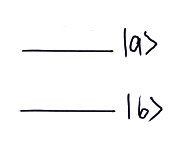
\includegraphics[width=0.4\linewidth]{fig/L4/2lvl}
	\caption{Atom's energy levels }
	\label{fig:2lvl}
\end{figure}

Mr. Hamiltonian is given by
\begin{equation}
	\hat{\mathscr{H}} = \frac{\hat{\vec{p}}^2}{2 m} + \hat{V} (\vec{r}).
\end{equation}
System has eigenstates which are given by equation
\begin{equation}
	\hat{\mathscr{H}} \ket{\psi} = E \ket{\psi}.
\end{equation}
So we have $E_a$ for $\ket{a}$ and $E_b$ for $\ket{b}$. After introducing electromagnetic field we have
\begin{equation}
	\hat{\mathscr{H}} = \frac{(\hat{\vec{p}} - \frac{e}{c} \vec{A})^2}{2m} + \hat{V}(\vec{r}) + e \varphi.
\end{equation}
Potentials are not determined and gauging may take place:
\begin{equation}
	\vec{A} \to \vec{A} + \frac{\hbar c}{e} \nabla \chi, \qquad \varphi \to \varphi - \frac{\hbar c}{e} \parder{\chi}{t}.
\end{equation}
After applying this gauging 
\begin{equation}
	\psi \to \psi e^{i \chi(\vec{r},t)}.
\end{equation}
Let a plane wave is falling 
\begin{equation}
	\vec{A} = \vec{A}_0 e^{i \vec{k}\vec{r} - i \omega t} = \vec{A}_0(t) e^{i \vec{k}\vec{r}}.
\end{equation}
Assume that characteristic scale of the system is such that 
\begin{equation}
	L \ll \lambda
	\label{eq:condition}
\end{equation}
is satisfied. Condition \eqref{eq:condition} is satisfied for lots of quantum systems. 
For example, visible light is $\lambda \sim 400 \div 800 \text{ нм}$, 
characteristic size of an atom is about $10^{-10} \text{ м}$, size of a quantum dot is about $10 \text{ нм}$. 

\begin{figure}[h!]
	\centering
	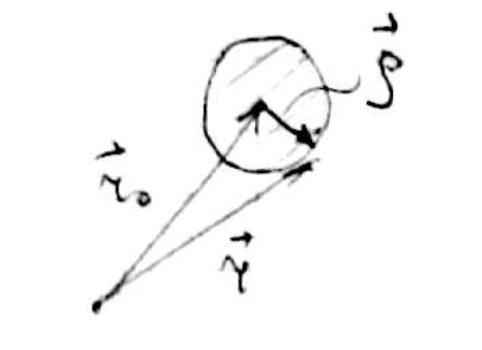
\includegraphics[width=0.4\linewidth]{fig/L4/simply}
	\caption{System}
	\label{fig:simply}
\end{figure}


Using this simplification we can $\vec{r}_0 \to \vec{r}$, where $\vec{r}_0$ is a vector of a centre of the system. More formaly this result may be achieved by expanding $\vec{A}$ near $\vec{r}_0$ in Taylor series:
\begin{equation}
	\vec{A} (\vec{r},t) \approx \vec{A}_0 (t) e^{i \vec{k} \vec{r}_0} \left( 1 + i \vec{k} \bm{\rho} \right) \approx \vec{A}_0 e^{i \vec{k} \vec{r}_0}.
\end{equation} 
So field does not change in space, but in time. Let us choose the system of axes so as to $\vec{r}_0 = 0$. It means that $\vec{A} \approx \vec{A}_0 (t)$. So
\begin{equation}
	\hat{\mathscr{H}} = \frac{1}{2m} \left( \hat{\vec{p}}  - \frac{e}{c} \vec{A}_0(t) \right)^2 + V (\vec{r}) + e \varphi.
\end{equation}
The standard choice it to use Coulomb gauging:
\begin{equation}
	\Div \vec{A} = 0, \qquad \varphi = 0.
\end{equation}
After that, using $\hat{\vec{p}} = -i \hbar \nabla$, we obtain
\begin{equation}
	\hat{\mathscr{H}} = - \frac{\hbar^2}{2m} \left( \nabla - \frac{i e}{\hbar c} \vec{A}_0  \right)^2 + V(\vec{r}).
\end{equation}
Lets introduce a new wave function $\widetilde{\psi} = \psi \underbrace{e^{- i \frac{e}{c \hbar} \vec{A}_0 \vec{r}}}_{\hookrightarrow = u}$. After that, the $ u^{\dagger} \hat{\mathscr{H}} u $ transformation will make an impulse shift.
\begin{equation}
	\hat{\mathscr{H}} \psi = \hat{\mathscr{H}} \widetilde{\psi} e^{i \frac{e}{c \hbar} \vec{A}_0 (t) \vec{r}}.
\end{equation}
We shall call $\vec{g} \myeq \frac{e}{c \hbar} \vec{A}_0 (t)$. After that lets consider
\begin{equation}
	\left( \nabla - i \vec{g} \right) \left( \nabla - i \vec{g} \right) \widetilde{\psi} e^{i \vec{g} \vec{r}} = \\ = \left( \nabla - i \vec{g} \right) \left( \nabla \widetilde{\psi}  \right) e^{i \vec{g} \vec{r}} = \left( \nabla^2 \widetilde{\psi} \right) e^{i \vec{g} \vec{r}}.
\end{equation}
Schroedinger equation gives us
\begin{equation}
	\hat{\mathscr{H}} \psi = i \hbar \parder{\psi}{t},
\end{equation}
\begin{equation}
	\underbrace{\left( - \frac{\hbar^2}{2m} \nabla^2 + V \right)}_{\hat{\mathscr{H}}_0} \widetilde{\psi} (\vec{r},t) = i \hbar \parder{\widetilde{\psi}}{t} - \hbar \vec{r} \cdot \parder{\vec{g}}{t} \widetilde{\psi}.
	\label{eq:tmp143}
\end{equation} 
Lets pay attention to  
\begin{equation}
	\parder{\vec{g}}{t} = \frac{e}{\hbar c} \parder{\vec{A}_0(t)}{t} = - \frac{e}{\hbar} \vec{E}(t).
\end{equation}
Using that we can rewrite \eqref{eq:tmp143} as
\begin{equation}
	\hat{\mathscr{H}}_0 \widetilde{\psi} - e \vec{r} \vec{E} \widetilde{\psi} = i \hbar \parder{\widetilde{\psi}}{t}.
\end{equation}
It's convenient to denote $\hat{\mathscr{H}}_1 \myeq - e \vec{r} \vec{E}$ --- a dipole energy in electric field, so finally
\begin{equation}
	\left( \hat{\mathscr{H}}_0 + \hat{\mathscr{H}}_1 \right) \widetilde{\psi} = i \hbar \parder{\widetilde{\psi}}{t}.
\end{equation}

Let us do an expansion of $\psi$ in eigenstates:
\begin{equation}
	\ket{\psi} = C_a(t) \ket{a} + C_b(t) \ket{b},
\end{equation}
where
\begin{equation}
	\hat{\mathscr{H}}_0 \ket{a} = E_a \ket{a}, \qquad \hat{\mathscr{H}}_0 \ket{b} = E_b \ket{b}.
\end{equation}
Beside $E_a - E_b = \hbar \omega_0$ --- the transition frequency. Let incident field be $\bm{\varepsilon} = \bm{\varepsilon}_0 \cos \omega t$, so $\hat{\mathscr{H}}_1 = - \vec{d} \cdot \bm{\varepsilon}$. Let define initial conditions at moment $t = 0$:
\begin{equation}
	\ket{\psi} \Big|_{t = 0} = \ket{b} \qquad \to \qquad
	\begin{matrix}
		C_a(0) = 0, \\
		C_b(0) = 1.
	\end{matrix}
\end{equation}
